\documentclass[12pt,a4paper]{article}
\usepackage[utf8]{inputenc}
\usepackage[T2A]{fontenc}
\usepackage[russian, english]{babel}
\usepackage{graphicx}
\usepackage{listings}
\begin{document}
\section{Постановка задачи}
Цели лабораторной работы:
\begin{enumerate}
    \item Язык SQL. Выборка данных с использованием операторов SELECT. WHERE. GROUP BY. HAVING. ORDER BY.
    \item Язык SQL. Объединения JOIN.
\end{enumerate}
\section{Получение данных}
Дамп базы данных IMDB. 

https://drive.google.com/open?id=1MYZbB21AFgFHSuoiNU\_I2xonnE4dX8pj
\begin{enumerate}
    \item \textbf{IMDB\_DB\_DUMP} - Полный дамп базы данных IMDB. Размер 7GB.
    \item \textbf{IMDB\_DB\_DUMP\_RATING} - Дамп базы данных IMDB в котором убрана информация про фильмы для которых нет рейтинга.
    \item \textbf{IMDB\_DB\_DUMP\_RATING\_SORT\_100K} - Дамп базы данных IMDB c информацией про фильмы из топ 100к в рейтниге.
    \item \textbf{IMDB\_DB\_DUMP\_RATING\_SORT\_10K} - Дамп базы данных IMDB c информацией про фильмы из топ 10к в рейтниге.
\end{enumerate} \par
Физическая модель дампа базы данных:
\begin{figure}[ht]
    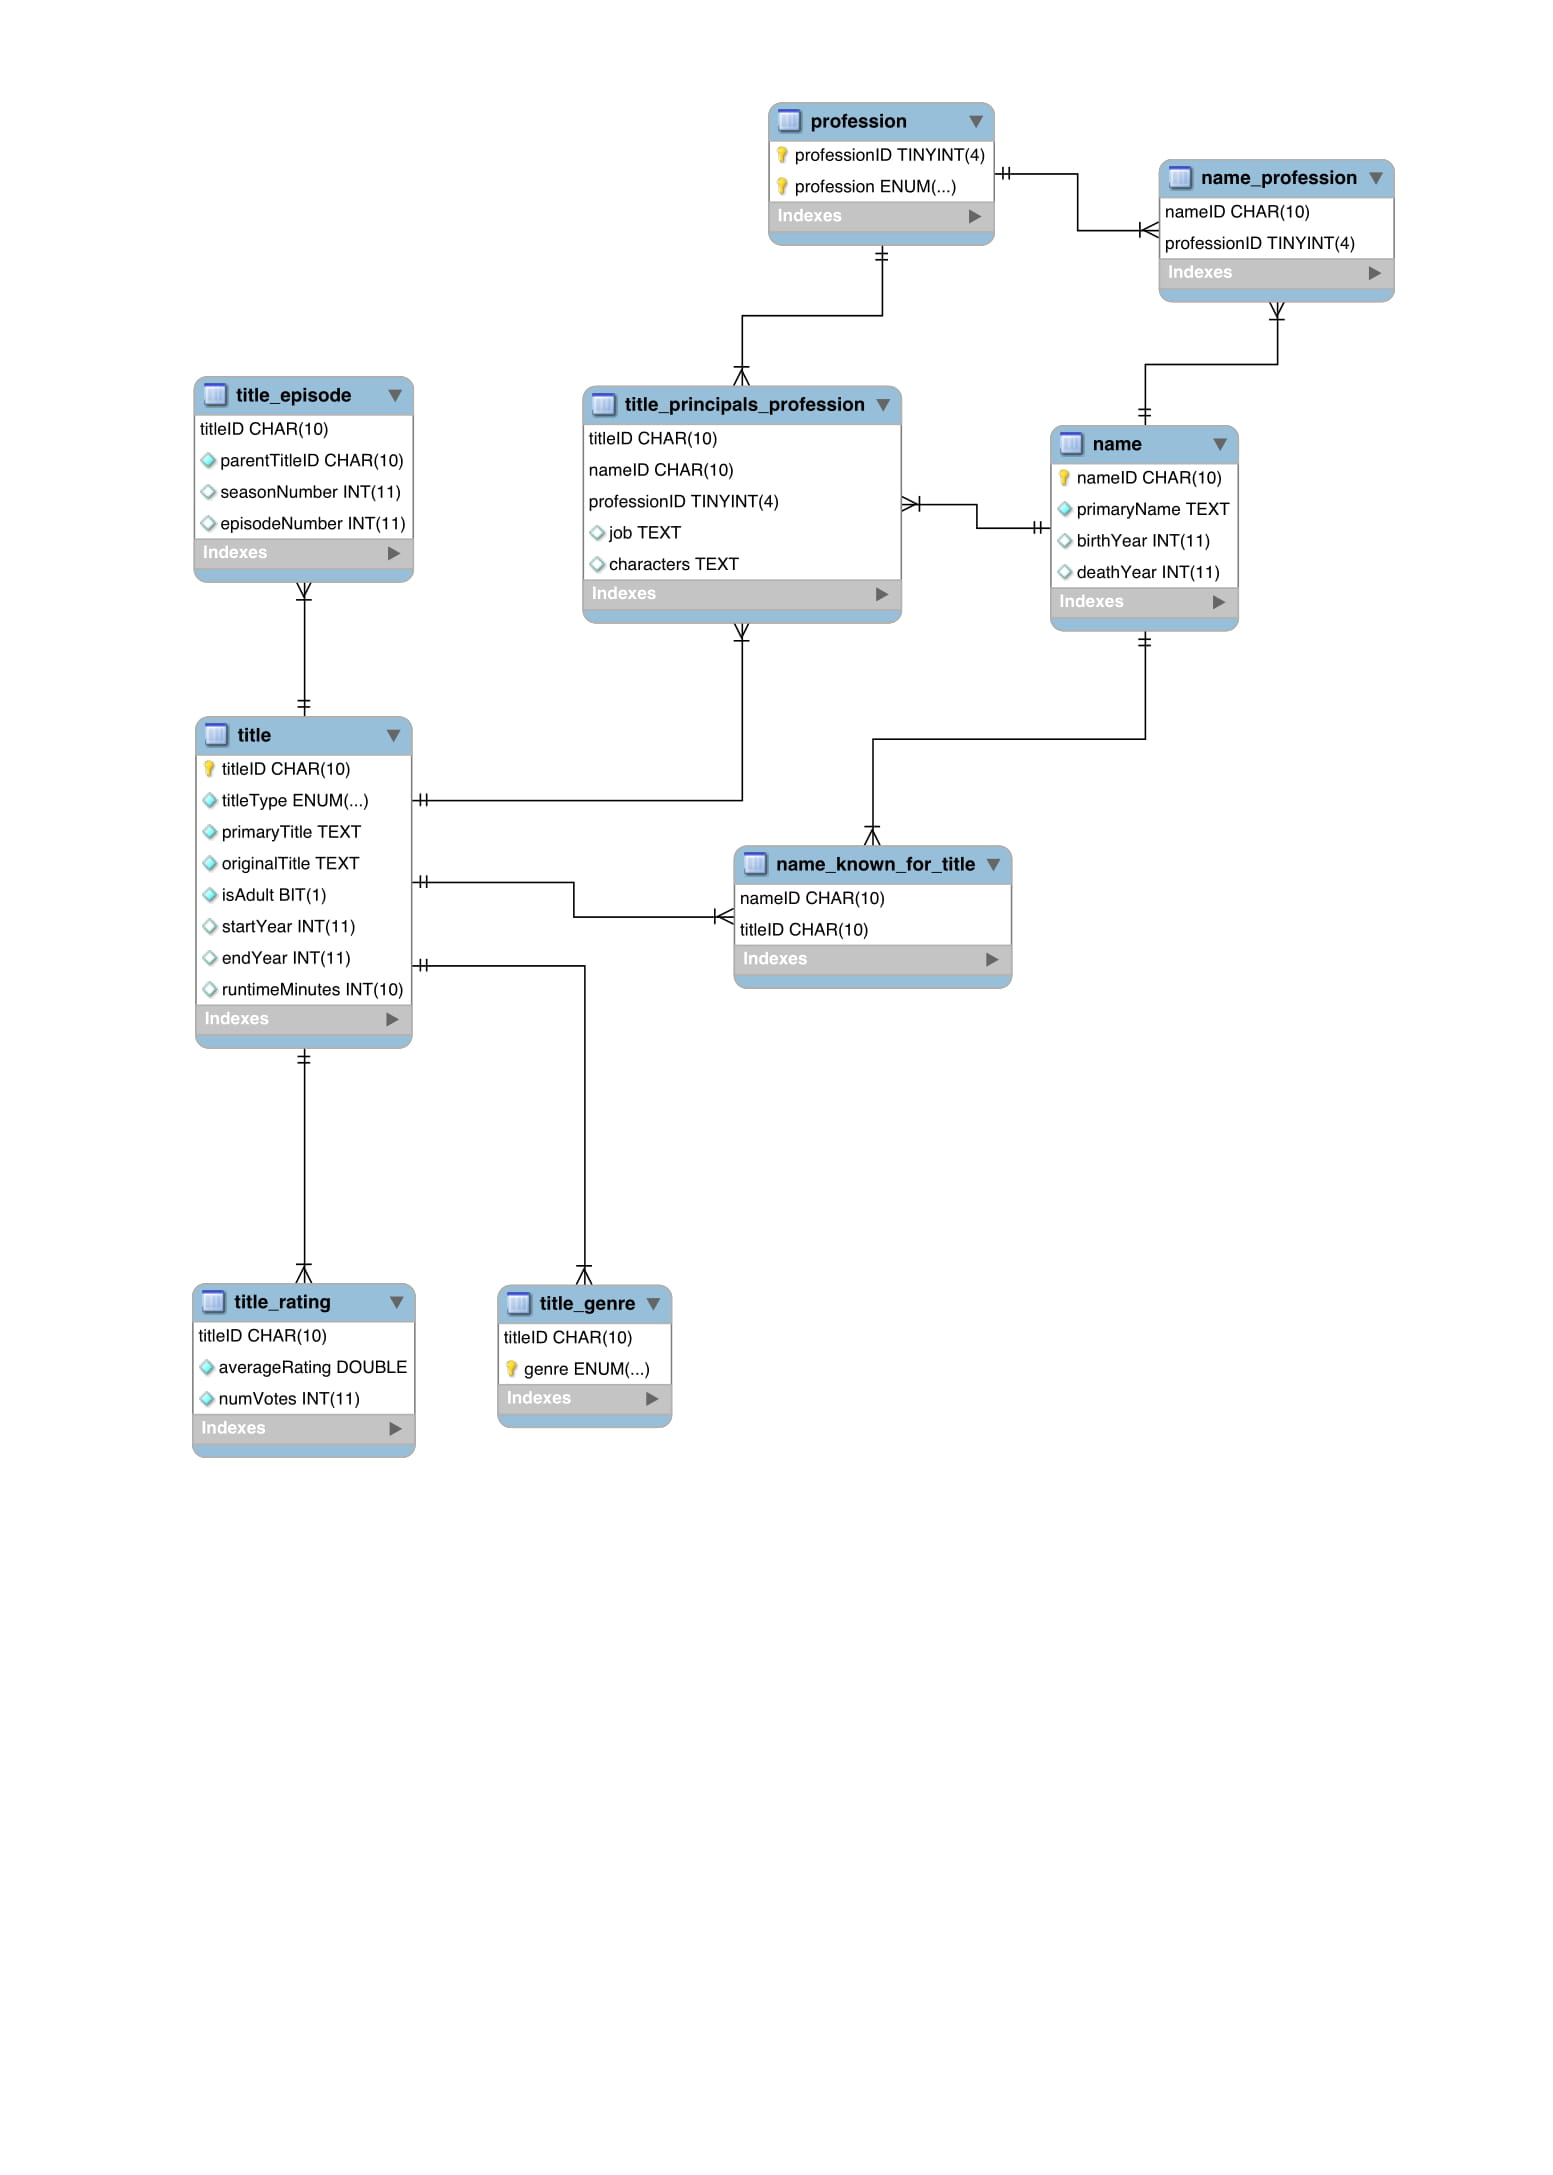
\includegraphics[width=\linewidth]{images/Lab3/IMDB_DB_Model.jpg}
    \caption{Physical model}
    \label{fig:Physical model}
  \end{figure}
\section{Запросы}
Получение всех фильмов отсортированных по рейтингу в порядке убывания.
\begin{lstlisting}[language=SQL]
SELECT originalTitle, titleType, averageRating, numVotes FROM title
INNER JOIN title_rating ON title.titleID = title_rating.titleID
ORDER BY numVotes DESC, averageRating DESC
LIMIT 10;
\end{lstlisting}
\begin{lstlisting}[basicstyle = \tiny\ttfamily, columns = fixed]
+---------------------------------------------------+-----------+---------------+----------+
| originalTitle                                     | titleType | averageRating | numVotes |
+---------------------------------------------------+-----------+---------------+----------+
| The Shawshank Redemption                          | movie     |           9.3 |  2149031 |
| The Dark Knight                                   | movie     |             9 |  2118625 |
| Inception                                         | movie     |           8.8 |  1883746 |
| Fight Club                                        | movie     |           8.8 |  1716980 |
| Pulp Fiction                                      | movie     |           8.9 |  1686388 |
| Forrest Gump                                      | movie     |           8.8 |  1653584 |
| Game of Thrones                                   | tvSeries  |           9.4 |  1596735 |
| The Matrix                                        | movie     |           8.7 |  1546559 |
| The Lord of the Rings: The Fellowship of the Ring | movie     |           8.8 |  1542044 |
| The Lord of the Rings: The Return of the King     | movie     |           8.9 |  1526805 |
+---------------------------------------------------+-----------+---------------+----------+
10 rows in set (0.47 sec)
\end{lstlisting}
Получение количества фильмов соответствующих жанру отсортированных по убыванию:
\begin{lstlisting}[language=SQL]
SELECT genre, COUNT(genre) as genre_count FROM title_genre
GROUP BY genre
ORDER BY genre_count DESC
LIMIT 10;
\end{lstlisting}
\begin{lstlisting}[basicstyle = \tiny\ttfamily, columns = fixed]
+-------------+-------------+
| genre       | genre_count |
+-------------+-------------+
| Drama       |     1692898 |
| Comedy      |     1316902 |
| Short       |      842509 |
| Documentary |      603245 |
| Talk-Show   |      587668 |
| Romance     |      576145 |
| Family      |      432405 |
| News        |      401786 |
| Reality-TV  |      319441 |
| Animation   |      313577 |
+-------------+-------------+
10 rows in set (3.99 sec)
\end{lstlisting}
Получение всех фильмов с заголовком Batman или Dark knight отсортированных по рейтингу.
\begin{lstlisting}[language=SQL]
SELECT title.titleID, originalTitle, averageRating, numVotes FROM title
INNER JOIN title_rating ON title.titleID = title_rating.titleID
WHERE originalTitle LIKE '%Batman%' OR originalTitle LIKE '%Dark Knight%' AND titleType = 'movie'
ORDER BY title_rating.numVotes DESC, title_rating.averageRating DESC
LIMIT 5
\end{lstlisting}
\begin{lstlisting}[basicstyle = \tiny\ttfamily, columns = fixed]
+-----------+------------------------------------+---------------+----------+
| titleID   | originalTitle                      | averageRating | numVotes |
+-----------+------------------------------------+---------------+----------+
| tt0468569 | The Dark Knight                    |             9 |  2118625 |
| tt1345836 | The Dark Knight Rises              |           8.4 |  1415027 |
| tt0372784 | Batman Begins                      |           8.2 |  1219308 |
| tt2975590 | Batman v Superman: Dawn of Justice |           6.5 |   587679 |
| tt0096895 | Batman                             |           7.5 |   318814 |
+-----------+------------------------------------+---------------+----------+
5 rows in set (0.48 sec)
\end{lstlisting}
Получить список людей ставших известными за фильм Batman(id='tt0468569');
\begin{lstlisting}[language=SQL]
SELECT primaryName FROM name_known_for_title 
INNER JOIN name ON name_known_for_title.nameID = name.nameID
WHERE titleID = 'tt0468569'
LIMIT 5
\end{lstlisting}
\begin{lstlisting}[basicstyle = \tiny\ttfamily, columns = fixed]
+-----------------+
| primaryName     |
+-----------------+
| Bob Cadigan     |
| Janice Buchanan |
| Brian Allen     |
| Kendis Rochlen  |
+-----------------+
4 rows in set (0.00 sec)
\end{lstlisting}
Получить актерский состав фильма Batman(id='tt0468569');
\begin{lstlisting}[language=SQL]
SELECT primaryName, profession FROM title_principals_profession
INNER JOIN name ON title_principals_profession.nameID = name.nameID
INNER JOIN profession ON profession.professionID = title_principals_profession.professionID
WHERE titleID = 'tt0468569'
\end{lstlisting}
\begin{lstlisting}[basicstyle = \tiny\ttfamily, columns = fixed]
+-------------------+------------+
| primaryName       | profession |
+-------------------+------------+
| Christian Bale    | actor      |
| Michael Caine     | actor      |
| Aaron Eckhart     | actor      |
| Bob Kane          | writer     |
| Heath Ledger      | actor      |
| David S. Goyer    | writer     |
| Christopher Nolan | director   |
| Jonathan Nolan    | writer     |
| Lorne Orleans     | producer   |
| Charles Roven     | producer   |
+-------------------+------------+
10 rows in set (0.00 sec)
\end{lstlisting}
\section{Используемые источники}
\begin{enumerate}
    \item https://dev.mysql.com/doc/refman/8.0/en/select.html
    \item https://dev.mysql.com/doc/refman/8.0/en/select-into.html
    \item https://dev.mysql.com/doc/refman/8.0/en/join.html
    \item https://dev.mysql.com/doc/refman/8.0/en/union.html
    \item https://dev.mysql.com/doc/refman/8.0/en/subqueries.html
\end{enumerate}
\end{document}